\chapter{SYSTEM DESIGN }

 \section{Use case model}
\begin{figure}[H]
    \centering
    \begin{tikzpicture}[
        actor/.style={font=\small, align=center},
        usecase/.style={ellipse, draw, align=center, text width=3.2cm, minimum height=1cm, font=\small},
        arr/.style={->, >=stealth, thick}
    ]
        % System boundary
        \draw[rounded corners, dashed] (1,-0.5) rectangle (9.5,12);
        \node at (5.25,12.4) {\textbf{AIRES System}};

        % Actors
        \node[actor] (cand) at (-1.5, 10) {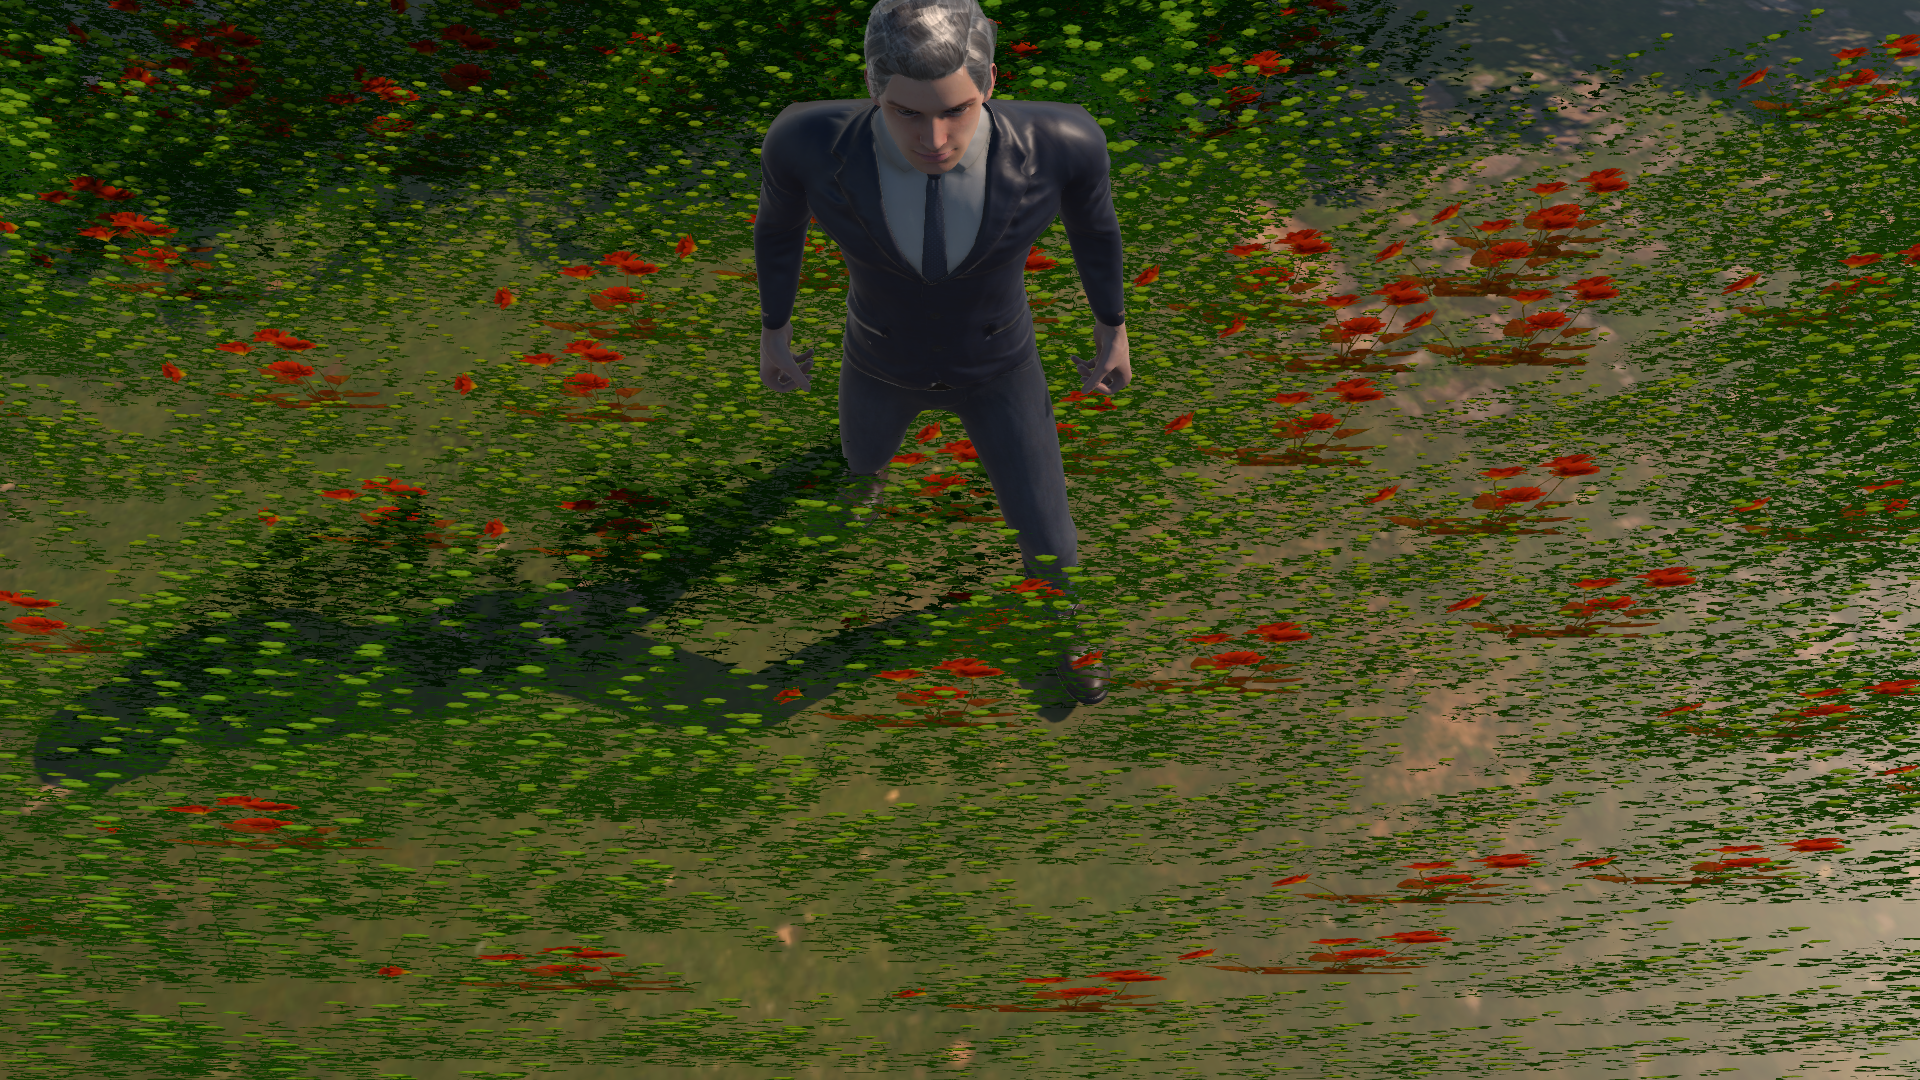
\includegraphics[width=0.5cm]{3rd_per.png}\\Candidate};
        \node[actor] (rec) at (12.5, 10) {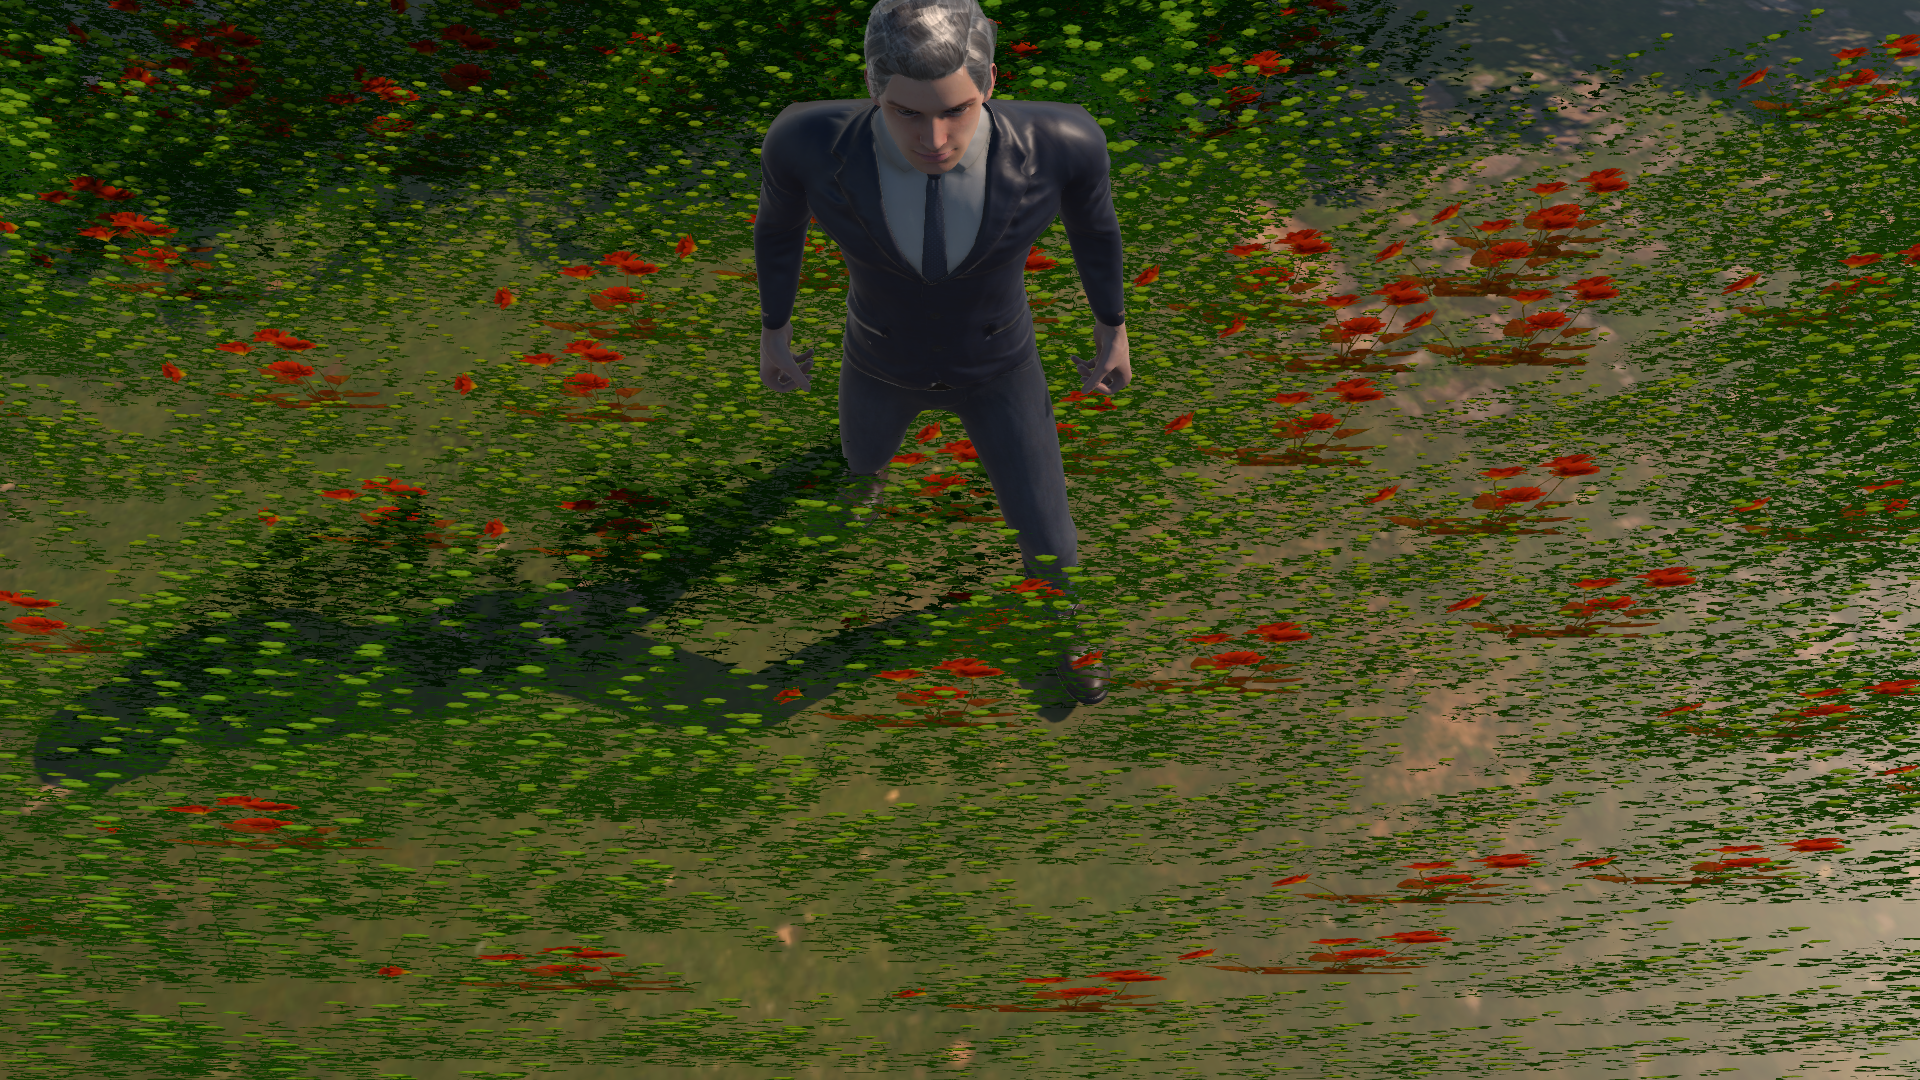
\includegraphics[width=0.5cm]{3rd_per.png}\\Recruiter};

        % Use cases - candidate
        \node[usecase] (uc1) at (4, 11.2) {Register / Login};
        \node[usecase] (uc2) at (4, 9.2) {Upload Resume};
        \node[usecase] (uc3) at (4, 7.2) {View AI Match Scores};
        \node[usecase] (uc4) at (4, 5.2) {View Skill Gap};
        \node[usecase] (uc5) at (4, 3.2) {Apply to Job};
        \node[usecase] (uc6) at (4, 1.2) {Track Application Status};

        % Use cases - recruiter
        \node[usecase] (uc7) at (7.5, 9.2) {Post / Edit / Delete Job};
        \node[usecase] (uc8) at (7.5, 7.2) {View Ranked Candidates};
        \node[usecase] (uc9) at (7.5, 5.2) {Update App Status};
        \node[usecase] (uc10) at (7.5, 3.2) {View Analytics};

        % Candidate connections
        \draw[arr] (cand) -- (uc1);
        \draw[arr] (cand) -- (uc2);
        \draw[arr] (cand) -- (uc3);
        \draw[arr] (cand) -- (uc4);
        \draw[arr] (cand) -- (uc5);
        \draw[arr] (cand) -- (uc6);

        % Recruiter connections
        \draw[arr] (rec) -- (uc1);
        \draw[arr] (rec) -- (uc7);
        \draw[arr] (rec) -- (uc8);
        \draw[arr] (rec) -- (uc9);
        \draw[arr] (rec) -- (uc10);
    \end{tikzpicture}
    \caption{Use Case Diagram -- AIRES}
    \label{fig:Use_case}
\end{figure}
The use case diagram illustrates the interactions between the two primary actors---Candidate and Recruiter---and the AIRES system. Both actors share the Register/Login use case. Candidates interact with resume management, job matching, skill gap analysis, application submission, and status tracking features. Recruiters interact with job posting management, candidate ranking, application status update, and analytics features.

 \section{Activity Diagram}
 \subsection{Candidate Workflow}
\begin{figure}[H]
    \centering
    \begin{tikzpicture}[
        node distance=0.7cm,
        act/.style={rectangle, rounded corners, draw, fill=blue!10, text width=3.5cm, align=center, minimum height=0.9cm, font=\small},
        dec/.style={diamond, draw, fill=yellow!20, text width=2.2cm, align=center, font=\scriptsize, aspect=2},
        arr/.style={->, >=stealth, thick},
        start/.style={circle, draw, fill=black, minimum size=0.4cm},
        stop/.style={circle, draw, fill=black, minimum size=0.4cm, double}
    ]
        \node[start] (s) {};
        \node[act, below=of s] (login) {Register / Login as Candidate};
        \node[act, below=of login] (upload) {Upload Resume (PDF/DOCX)};
        \node[dec, below=0.55cm of upload] (valid) {Valid File?};
        \node[act, right=2.5cm of valid] (error) {Show Error Message};
        \node[act, below=0.9cm of valid] (parse) {AI Parses Resume};
        \node[act, below=of parse] (view) {View Jobs with Match Scores};
        \node[act, below=of view] (apply) {Apply to Desired Job};
        \node[act, below=of apply] (track) {Track Application Status};
        \node[stop, below=of track] (e) {};

        \draw[arr] (s) -- (login);
        \draw[arr] (login) -- (upload);
        \draw[arr] (upload) -- (valid);
        \draw[arr] (valid) -- node[right, font=\scriptsize]{No} (error);
        \draw[arr] (error) |- (upload);
        \draw[arr] (valid) -- node[left, font=\scriptsize]{Yes} (parse);
        \draw[arr] (parse) -- (view);
        \draw[arr] (view) -- (apply);
        \draw[arr] (apply) -- (track);
        \draw[arr] (track) -- (e);
    \end{tikzpicture}
    \caption{Activity Diagram -- Candidate Workflow}
    \label{fig:activity_candidate}
\end{figure}
\subsection{Recruiter Workflow}
\begin{figure}[H]
    \centering
    \begin{tikzpicture}[
        node distance=0.7cm,
        act/.style={rectangle, rounded corners, draw, fill=green!10, text width=3.5cm, align=center, minimum height=0.9cm, font=\small},
        dec/.style={diamond, draw, fill=yellow!20, text width=2.2cm, align=center, font=\scriptsize, aspect=2},
        arr/.style={->, >=stealth, thick},
        start/.style={circle, draw, fill=black, minimum size=0.4cm},
        stop/.style={circle, draw, fill=black, minimum size=0.4cm, double}
    ]
        \node[start] (s) {};
        \node[act, below=of s] (login) {Register / Login as Recruiter};
        \node[act, below=of login] (post) {Post New Job Listing};
        \node[act, below=of post] (view) {View Ranked Candidate List};
        \node[act, below=of view] (status) {Update Application Status};
        \node[act, below=of status] (analytics) {Review Analytics Dashboard};
        \node[stop, below=of analytics] (e) {};

        \draw[arr] (s) -- (login);
        \draw[arr] (login) -- (post);
        \draw[arr] (post) -- (view);
        \draw[arr] (view) -- (status);
        \draw[arr] (status) -- (analytics);
        \draw[arr] (analytics) -- (e);
    \end{tikzpicture}
    \caption{Activity Diagram -- Recruiter Workflow}
    \label{fig:activity_recruiter}
\end{figure}
 \section{project Design}
 The system design of AIRES follows a component-driven, modular architecture aligned with the separation of concerns principle. The frontend is structured as a React SPA with distinct components for each feature area. The backend exposes a RESTful API consumed by the frontend. The design prioritizes a clean user experience, intuitive navigation, and data consistency across all views.\\\\
 The application is organized into two primary interaction layers: the public authentication layer (Login and Register screens) and the private, role-gated dashboard layer. Role-based routing ensures that candidates and recruiters are presented with entirely different interfaces upon authentication.

 \subsection{UI Design}
The AIRES user interface is designed with a premium, modern aesthetic. The login and registration screens feature a split-panel layout with a gradient background on one side and the authentication form on the other. The dashboard views use card-based layouts with subtle drop shadows and rounded corners, consistent with contemporary SaaS design patterns. Color-coded match score badges (green for high, orange for medium, red for low) provide immediate visual feedback to candidates. Recruiter dashboards use a tab-based navigation pattern to switch between Analytics, Jobs, and Candidates sections. All interactive elements feature smooth CSS transitions and hover effects to enhance the sense of responsiveness and polish.

\subsection{Component Architecture}
\medskip
The frontend codebase is organized into a set of focused, single-responsibility React components. The component hierarchy is as follows:\\\\
\noindent
The \textbf{App.jsx} component serves as the application root, managing the authenticated user state and rendering the React Router configuration. It seeds demo job data on first load if no jobs exist in localStorage.\\\\
\noindent
The \textbf{Login.jsx} and \textbf{Register.jsx} components handle user credential input and validation, executing role-based redirects upon successful authentication. Registration captures name, email, password, and role fields.\\\\
\noindent
The \textbf{CandidateDashboard.jsx} component orchestrates the candidate view by composing the ResumeUpload, ResumeInsights, My Applications, and JobList sub-components. It holds and distributes the parsed resume state across its children.\\\\
\noindent
The \textbf{RecruiterDashboard.jsx} component implements a tab-driven layout, rendering the Analytics, JobPost, or CandidateRanking component based on the active tab selection.\\\\
\noindent
The \textbf{ResumeUpload.jsx} component handles file selection, type validation, upload simulation, and AI parsing. It invokes a callback to update the parent's resume state on successful processing.\\\\
\noindent
The \textbf{JobList.jsx} component fetches available jobs, calculates match scores and skill gaps for each, presents a filtered and sorted job list, and handles job application submissions.\\\\
\noindent
The \textbf{CandidateRanking.jsx} component loads all applications, sorts them by match score, allows filtering by job, and exposes a status-change interface for each applicant.\\\\
\noindent
The \textbf{JobPost.jsx} component provides a form for creating and editing job postings and displays all currently active job listings with edit and delete controls.\\\\
\noindent
The \textbf{Analytics.jsx} component computes and displays recruiter statistics including totals and derived metrics such as shortlist rate and average applications per job.

\subsection{Data Model Design}
The core data entities in AIRES and their key attributes are described below.\\\\
\textbf{User Object:}
\begin{lstlisting}[style=csharpstyle]
{
  "id": "unique-user-id",
  "name": "Full Name",
  "email": "user@example.com",
  "password": "hashed-password",
  "role": "candidate" | "recruiter"
}
\end{lstlisting}

\textbf{Job Object:}
\begin{lstlisting}[style=csharpstyle]
{
  "id": "JOB-1001",
  "title": "Full Stack Developer",
  "requiredSkills": ["React", "Node.js", "MongoDB"],
  "postedAt": "2025-01-01T00:00:00.000Z"
}
\end{lstlisting}

\textbf{Application Object:}
\begin{lstlisting}[style=csharpstyle]
{
  "id": "unique-application-id",
  "jobId": "JOB-1001",
  "jobTitle": "Full Stack Developer",
  "candidateId": "unique-user-id",
  "candidateName": "Full Name",
  "candidateEmail": "user@example.com",
  "appliedAt": "2025-01-02T00:00:00.000Z",
  "status": "Applied" | "Shortlisted" | "Rejected",
  "matchScore": 75
}
\end{lstlisting}

\textbf{Resume Data Object:}
\begin{lstlisting}[style=csharpstyle]
{
  "userId": "unique-user-id",
  "fileName": "resume.pdf",
  "uploadedAt": "2025-01-01T00:00:00.000Z",
  "parsedData": {
    "skills": ["JavaScript", "React", "Node.js"],
    "education": [{ "degree": "B.Tech", "field": "CS", "year": "2023" }],
    "experience": [{ "title": "Intern", "company": "Tech Corp" }]
  }
}
\end{lstlisting}

\subsection{Background Score Design}
The AIRES scoring model uses a weighted, substring-based skill matching approach. All skill strings are normalized to lowercase before comparison to eliminate case sensitivity issues. A candidate skill is considered to satisfy a job requirement if either string is a substring of the other, accommodating common shorthand variations (e.g., ``JS'' vs ``JavaScript'' can be handled by extending the normalization dictionary in future versions). The overall match score is a linear measure, giving equal weight to each required skill. Future enhancements could incorporate weighted skill importance rankings defined by the recruiter.

\subsection{Sound Effects}
Not applicable to the AIRES web application. AIRES is a silent, browser-based platform designed for professional use in a work environment. Audio notifications are not included in the current scope.

\subsection{Question Design}
Not applicable to the AIRES project. AIRES does not use quiz or question-based mechanics. Skill matching is performed automatically based on the AI-parsed resume data without user interaction at the matching stage.

